% !TEX root = ../CategoricalCoDesign.tex
\section{Thinking about how things transform into each other}

\subsection{Category theory helps reasoning about interfaces and transformations}
\todo{Arrows should agree with profunctors notation}

We argue that all the concepts of formal engineering design discussed in the
previous section can be naturally described in the language of category theory.

We will start with a simple example.

In an electric car, electric power is turned by the engine into rotational
motion of the axle, and then the rotational motion is converted into
translational motion by the wheels and their friction with the road.

In this simple setting, we can identify the key systems and subsystems: Car,
engine, axle, wheels, and road.

We can identify the functionality/resources of interest as: Electric
power, rotational motion, and translational motion. Note that each of these quantities
plays a dual role: For example, the rotational motion is something which is
produced by the motor, so it is a functionality for the motor, while it
is a resource for axle/wheels, because they need it to provide translational motion.

For a first qualitative description of the scenario, we might choose to just
keep track of what functionality/resource is converted into what.

For this qualitative description, we can draw a diagram in which each resource
is a point (\cref{fig:e1}).

\begin{figure}[h!]
    \centering
    \includesag{30_dpcatfig_e1}
    \caption{\label{fig:e1}}
\end{figure}

Furthermore, we can draw an arrow between two resources if we can obtain one
from the other. In the example, we have described how power becomes rotational
motion (arrow $\mathsf{converter}$) and how rotational motion becomes translational motion
(arrow $\mathsf{wheel}$) (\cref{fig:e2}).

\begin{figure}[h!]
    \centering
    \includesag{30_dpcatfig_e2}
    \caption{\label{fig:e2}}
\end{figure}

In this representation, the arrows are the components of the system.
We will learn how to compose these arrows according to the rules of category theory.

If we use the semantics that an arrow from resource $X$ to resource $Y$ means ``Having $Y$ is
enough to obtain $X$'', then, since $Y$ is enough for $Y$, we can add a self-loop for each
resource (\cref{fig:e3}). We will call the self-loops \emph{identities} (\cref{fig:e3}).

\begin{figure}[h!]
    \centering
    \includesag{30_dpcatfig_e3}
    \caption{\label{fig:e3}}
\end{figure}

Furthermore, we might consider the idea of composition of arrows: if from $Y$ we
can get $X$ and from $Z$ we can get $Y$, then from $Z$ we can get $X$. In our
example, if the arrows $\mathsf{converter}$ and $\mathsf{wheel}$ exist, then also the arrow ``$\mathsf{converter}$ then $\mathsf{wheel}$''
exists~(\cref{fig:e4}).


\begin{figure}[h!]
    \centering
    \includesag{30_dpcatfig_e4}
    \caption{\label{fig:e4}}
\end{figure}


A ``category'' is nothing more than this: It is an abstract mathematical
structure whose two primitive notions are objects and arrows between objects.
The following is the formal definition.

\begin{shaded}
\begin{definition}[Category] \label{def:categorymain}
A \emph{category} $\CatC$ is defined by describing four components: the
category's \emph{objects}, the category's \emph{morphisms},
the \emph{identities} and the \emph{composition operations}. More precisely,
a category consists of:
\begin{compactenum}
\item \emph{Objects}: A collection $\ObC$, whose elements are called \emph{objects}.
\item \emph{Morphisms}: For every pair of objects $X, Y\in\ObC$, there is
a way to define the set $\HomC(X, Y)$, which is called the ``hom-set from
$X$ to $Y$''. The elements of this set are called \emph{morphisms}.
\item \emph{Identity morphism}:  For each object $X$, there is
an element $\id_X \in \HomC(X,X) $ which is called \emph{the identity
morphism in $X$}.
\item \emph{Composition operation}: There is a way to define the composition
of two morphisms. Given a morphism $f \in  \HomC(X,Y) $ and a morphism $g \in \HomC(Y, Z)$, then
there exists a morphism $f\then g$ in $\HomC(X, Z)$.

In addition, there are two properties that must hold:

\begin{compactenum}
    \item Unitality: For a morphism $f\in\Hom(X,Y)$: 
    \begin{equation}
        \id_X \then f=f \then \id_Y.
    \end{equation}
    \item Associativity: The composition is associative, in the sense that for $f\in \HomC(X,Y)$, $g\in \HomC(Y,Z)$, and $h\in \HomC(Z,W)$:
    \begin{equation}
        (f\then g)\then h= f \then (g \then h).
    \end{equation}
\end{compactenum}

\end{compactenum}
\end{definition}
\end{shaded}



\AC{ Given that this is the first example of a category, let's list explicitly
the category that we are using. (wheels, converters, energy, etc.) }

The properties of a category allow us to save some ink in the drawing the
corresponding graph:
\begin{compactitem}
\item We do not need to draw the identity arrows from one object to itself, because they always exist. (However, we will see how there might be multiple such loops.)
\item  Whenever there are arrows $A\to B \to C$, we will not need to draw the arrows composition, because it always exists.
\end{compactitem}

With these conventions, we can just draw the arrows~$f$ and~$g$ in the diagram,
and the rest of the diagram is implied (\cref{fig:e5}). Particularly, this example corresponds to the category $\CatC$ specified by 
\begin{itemize}
    \item $\Ob_\CatC=\{\text{electric power},\text{rotational motion},\text{translational motion}\}$.
    \item E.g., we have morphisms $\mathsf{converter}$, $\mathsf{wheel}$, and $\mathsf{wheel}\text{ then }\mathsf{converter}$.
\end{itemize}

\begin{figure}[h!]
    \centering
    \includesag{30_dpcatfig_e5}
    \caption{\label{fig:e5} The grey arrows are implied by the properties
    of a category.}
\end{figure}

\todo{move the following to the currency subsection. Check the direction of the arrows!}  

We can slightly expand this example by noting the inverse transformations. In an electric car
it is possible to regenerate power; that is, we can obtain rotational motion of the wheels from
translational motion (via $\mathsf{move}$), and then convert the rotational motion into electric
power (via $\mathsf{dynamo}$)~(\cref{fig:e6}).

\begin{remark}
We denote map composition in a somewhat unusual way---sometimes preferred by category-theorists and computer scientists---namely in \emph{diagrammatic order}. That is, given $f\colon A\to B$ and $g\colon B\to C$, we denote their composite by $(f\then g)\colon A\to C$, pronounced ``$f$ then $g$'' rather than the more typical $g\circ f$ (``$g$ after $f$'').

Composition of maps is unital and associative: for any $f\colon A\to B$, $g\colon B\to C$, and $h\colon C\to D$, we have
\begin{equation}
(\id_A\then f)=f=(f \then \id_B)\qquad\text{and}\qquad f\then (g\then h)=(f\then g)\then h.
\end{equation}
\end{remark}

\begin{figure}[h!]
    \centering
    \includesag{30_dpcatfig_e6}
    \caption{\label{fig:e6}}
\end{figure}

These arrows are not necessarily the same arrows as before; there might be different processes
involved.

\begin{figure}[h!]
    \centering
    \includesag{30_dpcatfig_e7}
    \caption{\label{fig:e6-together}}
\end{figure}

Given the semantics of the arrows, all compositions of arrows exist, even if they are not drawn
explicitly. For example, we can consider the composition~$f\then g \then k \then h$, which
converts electric power into rotational motion into translational motion, then back to
rotational motion and electric power. This is an arrow that has the same head and tail as the
identity on electrical power~(\cref{fig:e8}). However, the arrows are not necessarily the same. In fact, we know that if these are physical systems, there will be some loss for the many conversions.

\begin{figure}[h!]
    \centering
    \includesag{30_dpcatfig_e8}
    %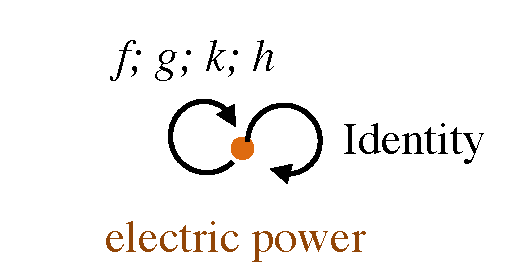
\includegraphics[scale=0.33]{dpcatfig_e8}
    \caption{\label{fig:e8}}
\end{figure}

In fact, it is important to recognize that there might be two or more distinct
arrows between two resources~(\cref{fig:e9}). Each arrow between $X$ and $Y$ represents a different way  to obtain~$X$ from~$Y$. This is what will make category theory powerful enough to reason about design.


\begin{figure}[h!]
    \centering
    \includesag{30_dpcatfig_e9}
    \caption{\label{fig:e9}}
\end{figure}

The directionality of the arrows is also important. While the convention of
which resource is the tail and which the head is just a typographic convention,
it might be the case that we know how to convert one resource into another, but
not vice versa.

\cref{fig:e10} shows an example of a diagram that describes a process which is definitely
not invertible.

\begin{figure}[h!]
    \centering
    \includesag{30_dpcatfig_e10}
    \caption{\label{fig:e10}}
\end{figure}
\subsection{The currency category}
\todo{For later - this will be more discursive. Definitions can be less formal. Symbols too heavy.
Will put nice pictures.}
\AC{I think here we can go to the incremental step of describing a category
in which the resources are isomorphic to real numbers. Before, we say
that fghk is not the identity, but really, if the resources are bool then fghk=identity.}
In this section, we consider as an example the category of currency exchangers $\mathbf{Curr}$. To introduce what currencies are, we need the notion of units.
\begin{definition}[Real with units]
    Define $\mathbb{R}_\mathsf{g}$ to be the set of real numbers $\mathbb{R}$ with unit $\mathsf{g}$. Given $\unit[p]{\mathsf{a}} \in \mathbb{R}_\mathsf{a}$ and $\unit[q]{\mathsf{b}}\in \mathbb{R}_\mathsf{b}$, define
    \begin{equation}
    \begin{aligned}
    \cdot \colon \mathbb{R}_\mathsf{a} \times \mathbb{R}_\mathsf{b} &\to \mathbb{R}_\mathsf{ab}\\
    \tup{\unit[p]{\mathsf{a}},\unit[q]{\mathsf{b}}}&\mapsto r\coloneqq \unit[p\cdot q]{\mathsf{ab}}.
    \end{aligned}
    \end{equation}
    Furthermore, note that two objects can be summed if and only if they share the same units. Note that from now on we will say $p\in \mathbb{R}_\mathsf{g}$ to mean $\unit[p]{\mathsf{g}}$, $p\in \mathbb{R}$.
\end{definition}

Consider two currencies, $\mathsf{C,D}$. A currency exchanger from $\mathsf{C}$ to $\mathsf{D}$ can be expressed as a pair $\tup{a,b}$, $a\in {\mathbb{R}_{>0}}_ {\frac{\mathsf{D}}{\mathsf{C}}}$ and $b\in {\mathbb{R}_{\geq 0}}_ {\mathsf{D}}$. The pair specifies an affine function of the form
\begin{equation}
        \begin{aligned}
        \mathsf{CE}\colon \mathbb{R}_\mathsf{C}&\to \mathbb{R}_\mathsf{D}\\
        \unit[p]{\mathsf{C}}&\mapsto \unit[q]{\mathsf{D}} \coloneqq a\cdot \unit[p]{\mathsf{C}} -b,
        \end{aligned}
    \end{equation}
   where $a$ represents the exchange rate from $\mathsf{C}$ to $\mathsf{D}$, and $b$ represents the fixed commission of the currency exchanger. Note that one can define the identity currency exchanger, $\tup{1,0}$, which is equivalent to not change the money. As an example, consider three currency exchange companies $\mathsf{ExchATM}$, $\mathsf{MoneyLah}$, and $\mathsf{Frankurrencies}$, which operate on several currencies (\cref{tab:currencycompanies}).
\begin{table}[h]
    \centering
    \begin{tabular}{c|c|c|c}
         operation name& details &$a$ (exchange rate)&$b$   (fixed commission)  \\
         $A$&USD to CHF&\unitfrac[0.95]{CHF}{USD}&\unit[2.0]{CHF}\\
         $B$&CHF to USD&\unitfrac[1.05]{USD}{CHF}&\unit[1.5]{USD}\\
         $C$&USD to SGD&\unitfrac[1.40]{SGD}{USD}&\unit[1.0]{SGD}    \end{tabular}\\[+5pt]
         \begin{tabular}{c|c|c|c}
         operation name& details &$a$ (exchange rate)&$b $ (fixed commission)  \\ $D$&USD to CHF&$\unitfrac[1.0]{CHF}{USD}$&\unit[1]{CHF}\\
         $E$&SGD to USD&\unitfrac[0.72]{USD}{SGD}&\unit[3.0]{USD}
    \end{tabular}\\[+5pt]
    \begin{tabular}{c|c|c|c}
         operation name& details &$a$ (exchange rate)&$b $ (fixed commission)  \\
        $F$& EUR to CHF&\unitfrac[1.2]{CHF}{EUR}&\unit[0]{CHF}\\
        $G$& CHF to EUR&\unitfrac[1.0]{EUR}{CHF}&\unit[1]{EUR}
    \end{tabular}
    \caption{Three currency exchange companies operating different currencies.
    }
    \label{tab:currencycompanies}
\end{table}

We can represent this information as a graph, where the nodes are the currencies and the edges are particular exchange operations (\cref{fig:currencygraph}).

\begin{figure}[h]
\begin{center}
    \begin{tikzcd}[column sep = 5cm, row sep = 3cm]
    \text{USD}\arrow[bend left=20, r,"A"]\arrow[bend right=20, r,"D",swap] 
    \arrow[d,bend left=20,"C"]
    &\text{CHF}
    \arrow[d,bend left=20,"G"]
    \arrow[l,"B"]\\
    \text{SGD}\arrow[u,bend left=20,"E"]&
    \text{EUR}
    \arrow[u,bend left=20,"F"]
    \end{tikzcd}
\end{center}
\caption{Three currency exchange companies operating different currencies as a graph \label{fig:currencygraph}}
\end{figure}

The graph representation seems enough to describe this as a category, where the objects are the currencies (USD,CHF,EUR, and SGD), the morphisms are the different exchange operations, and the identity morphisms are identity currency exchangers. However, to properly define this category, we need to define composition and prove that the category is closed with respect to it. Given three currencies $\mathsf{X,Y,Z}$, a currency exchanger $\tup{a,b}$ from $\mathsf{X}$ to $\mathsf{Y}$, and a currency exchanger $\tup{c,d}$ from $\mathsf{Y}$ to $\mathsf{Z}$, one can define their composition as
\begin{equation}
\begin{aligned}
\label{eq:currencycomp}
    \tup{a,b}\then \tup{c,d}&=\tup{c\cdot a,c\cdot b+d}\\
    &=\tup{e,f}.
\end{aligned}
\end{equation}
Note that the result of the composition of currency exchangers is a currency exchanger: This is closure. Finally, we need to check unitality and associativity for composition. Given a currency exchanger $\tup{a,b}$ from $\mathsf{X}$ to $\mathsf{Y}$ one has
\begin{equation}
    \begin{aligned}
    \tup{1,0}\then \tup{a,b}&=\tup{a,b}\then \tup{1,0}\\
    &=\tup{a,b},
    \end{aligned}
\end{equation}
which is unitality. Furthermore, given a currency exchanger $\tup{c,d}$ from $\mathsf{Y}$ to $\mathsf{Z}$ and a currency exchanger $\tup{e,f}$ from $\mathsf{Z}$ to $\mathsf{W}$, one has
\begin{equation}
    \begin{aligned}
    (\tup{a,b}\then \tup{c,d})\then \tup{e,f}&=\tup{a,b}\then( \tup{c,d}\then \tup{e,f})\\
    &=\tup{eca, ecb+ed+f},
    \end{aligned}
\end{equation}
which is associativity.
We are now ready to properly define the category of currency exchangers $\mathbf{Curr}$.

\begin{definition}[Category of currencies]
    The category of currencies $\mathbf{Curr}$ is specified by:
    \begin{compactenum}
        \item \emph{Objects:} $\Ob_\mathbf{Curr}$ is a collection of currencies.
        \item \emph{Morphisms:} Given two currencies $\mathsf{C},\mathsf{D}\in \Ob_{\mathbf{Curr}}$, morphisms between them are currency exchangers $\tup{a,b}$ from $\mathsf{C}$ to $\mathsf{D}$. 
        \item \emph{Identity morphism:} Given an object $C\in \Ob_\mathbf{Curr}$, the identity morphism is given by the currency exchanger $\tup{1,0}$.
        \item \emph{Composition of morphisms:} The composition of morphisms is given by composition of currency exchangers.
    \end{compactenum}
\end{definition}

The category Curr represents the set of all possible currency exchangers that could
ever exist. However, in this set there would be very irrational agents. For example, there is a currency exchanger that given 1 USD, will give you back 2 USD, or even not giving you back any money. This highlights a recurring topic: often mathematicians will be happy to define a broader category of objects, while, in practice, the engineer will find himself thinking about a more constrained set of objects. Particularly, one would like to find the best conversions, which can be expressed as \emph{pareto fronts}, since they are given as tuples $\tup{a,b}$. To do so, one only needs to iterate a finite number of times, since the optimal path (conversion morphism), if such a morphism exists, will never pass through the same currency more than once. This is valid if we assume the action of converting back and forth the same currency to have a cost (through the commission) different from 0. To see this, consider three currencies $\mathsf{A,B,C}$, a currency exchanger from $\mathsf{A}$ to $\mathsf{B}$  $\tup{a,b}$, a currency exchanger from $\mathsf{B}$ to $\mathsf{C}$ 
$\tup{c,d}$, and a currency exchanger from $\mathsf{C}$ to $\mathsf{A}$ $\tup{e,f}$. The composition of the currency exchangers reads:
\begin{equation}
\tup{\underbrace{eca}_{\diamond}, \underbrace{ecb+ed+f}_{\star}}
\end{equation}
Assuming $e=a^{-1}$ (i.e., an exchange rate direction is not more profitable than the other), $\star\neq 0$, because of the commissions. This shows that there are multiple morphisms from $\mathsf{A}$ to $\mathsf{A}$, and that the identity morphism is the most convenient one.


\AC{(Note, don't write: if bias is 0, then take the log of conversion rates, and they add: solve using Dijkstra.)}




